\chapter{变分法和Euler-Lagrange 方程}

\section{线性泛函}

若泛函$J[u,v]$满足下列条件
\begin{enumerate}[itemindent=2em]
    \item $J[u,v]=J[v,u]$;
    \item $J[\alpha_1 u_1+\alpha_2 u_2,v]=\alpha_1 J[u_1,v]+\alpha_2 J[u_2,v]$;
\end{enumerate}

则称$J[u,v]$为\textbf{对称双线性泛函},如果只满足线性性,则称为\textbf{双线性泛函},若$u=v$,则$J[u,u]$称为\textbf{二次泛函},如若只有一个参数$J[v]$,则称为\textbf{线性泛函}。


\section{最速下降线}

这是历史上最早出现的变分法问题之一,通常被认为是变分法历史的起点。该问题由伽利略于1630年提出来,1638年由系统研究过这个问题,但是他给出的结果不对。
认为这条曲线是一个圆弧。对变分法实质性的研究是约翰·伯努利在1696年在《教师学报》上写给他哥哥雅各布·伯努利的一封公开信中征求问题的解开始的。问题的提法是
:\textsl{设A和B是铅直平面上不在同一直线上的亮点,在所有连接$A$和$B$两点的平面曲线中,求一条曲线,使得仅仅受到重力加速度作用的、初速度为零的质点从$A$
到$B$沿这条曲线运动所需时间最短}。欧拉首先详尽的阐述了这个问题。他的贡献始于1733年,他的《变分原理》(Elementa Calculi Variationum)寄予了这门科学这个名字。欧拉对这个理论的贡献非常大。
,勒让德(1786)确定了一种方法,但在对极大和极小的区别不完全令人满意。牛顿和莱布尼茨也是在早期关注这一学科,对于这两者的区别Vincenzo Brunacci(1810)、高斯(1829)、泊松(1831)、Mikhail Ostrogradsky(1834)、和雅可比(1837)都曾做出过贡献。Sarrus(1842)的由柯西(1844)浓缩和修改的是一个重要的具有一般性的成就。Strauch(1849)、Jellett(1850)、Otto Hesse(1857)、Alfred Clebsch(1858)、和Carll(1885)写了一些其他有价值的论文和研究报告,但可能那个世纪最重要的成果是Weierstrass所取得的。他关于这个理论的著名教材是划时代的,并且他可能是第一个将变分法置于一个稳固而不容置疑的基础上的。1900年希尔伯特发表的23个问题中的第20和23个问题促进了其更深远的发展。

在20世纪希尔伯特、埃米·诺特、列奥尼达·托内利、昂利·勒贝格和雅克·阿达马等人做出重要贡献。Marston Morse将变分法应用在莫尔斯理论中。Lev Pontryagin、Ralph Rockafellar和Clarke广义变分法最优控制理论发展了新的数学工具。

现在我们重新阐述这个问题
\begin{framed}
    \begin{question}
        设A和B是铅直平面上不在同一直线上的亮点,在所有连接$A$和$B$两点的平面曲线中,求一条曲线,使得仅仅受到重力加速度作用的、初速度为零的质点从$A$
            到$B$沿这条曲线运动所需时间最短
    \end{question}
\end{framed}

\begin{figure}[H]
    \centering
    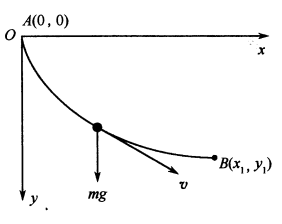
\includegraphics[scale=0.6]{figures/chapter3/最速下降线.png}
    \caption{最速下降线}
\end{figure}

我们的目的是找出一个关于时间函数$T$的表达式,并求其最小值。运动过程仅收到重力加速度
\begin{equation}
    mgy=\frac{1}{2}mv^2\ \Rightarrow\ v=\sqrt{2gy}
\end{equation}

引入时间变量
\begin{equation}
    v=\frac{ds}{dt}=\frac{\sqrt{dx^2+dy^2}}{dt}=\sqrt{1+y'^2}\frac{dx}{dt}
\end{equation}

整理两个式子得到关于时间的函数
\begin{equation}
    T=\int_{0}^{x}\sqrt{\frac{1+y'^2}{2gy}}dx
\end{equation}

$T$是关于$y(x)$的一个函数,像这种输入是函数,输出是数的函数,称为\textbf{泛函},问题是是使的这个$T$最小化,
也就是泛函极值问题。

\section{泛函极值问题}

设$F(x,y(x),y'(x))$是三个独立变量$x,y(x),y'(x)$在区间$[x_0,x_1]$上的已知函数,且二阶连续可微,
则
\begin{equation}
    J[y(x)]=\int_{x_0}^{x_1}F(x,y(x),y'(x))dx
\end{equation}

称为\textbf{最简积分型泛函},也称\textbf{最简泛函}或\textbf{价值泛函}。泛函$J[y'(x)]$称为
\textbf{泛函形式}或\textbf{变分积分},被积函数$F$称为\textbf{泛函的核函数}或者\textbf{变分被积函数}或者
\textbf{拉格朗日函数}。

因此,求泛函的极值即是求$\{y(x)|x\in X\}\xrightarrow{J} \mathcal{R}$下使的$J[\cdot]$取最值的$y(x)$。

\section{一阶变分}

变分法的主要思想是微小摄动,假设$y(x)$是使的泛函$J[y(x)]$最小的曲线,那么
在此之上增加任意摄动都会使得泛函增大。

在$y=y(x)$的\textsl{一阶领域}\footnote{《变分法基础》老大中. 定义\\ \hspace*{2em}\textbf{n阶领域}:函数$y(x)$在区间上$n$阶距离小于正数$\delta$的函数$y(x)$所组成的集合\\ \hspace*{2em}\textbf{n阶距离}:两个函数$0$到$n$阶导数之差的绝对值的最大值,$\max\limits_{0\leqslant i\leqslant n}\max\limits_{a\leqslant x\leqslant b}|y^{(i)}(x)-y_0^{(i)}(x)|$}内,
任取$y=y_1(x)$,
\begin{equation}
    \delta y=y_1(x)-y(x),\ \ \ \ \delta y'=y'_1(x)-y'(x) 
\end{equation}

考虑给到泛函$J[\cdot]$摄动$\delta y$的变化量为
\begin{equation}
    \begin{aligned}
         \Delta J&=J[y_1(x)]-J[y(x)]=J[y(x)+\delta y]-J[y(x)]\\
        &=\int_{x_0}^{x_1}[F(x,y+\delta y,y'+\delta y')-F(x,y,y')]dx
    \end{aligned}
\end{equation}

由多元函数的\textsl{泰勒中值定理}得
\begin{equation}
    F(x,y+\delta y,y'+\delta y')-F(x,y,y')=\overline{F}_y\delta y+\overline{F}_{y'}\delta y'
\end{equation}

其中$\overline{F}_{y}\delta y$表示$F$对$y$的一阶导数在$(x,\overline{y}(x),\overline{y}'(x))$处的值,其中$y(x)\leqslant \overline{y}(x)\leqslant y_1(x)$,$\overline{F}_{y'}\delta y'$对$y'$的一阶导数在$(x,\overline{y}(x),\overline{y}'(x))$处的值,其中$y(x)\leqslant \overline{y}(x)\leqslant y_1(x)$。
因此

\begin{equation}
    \begin{aligned}
        & |\overline{y}(x)-y(x)|<d_1[y_1(x),y(x)]\\
        & |\overline{y}'(x)-y'(x)|<d_1[y'_1(x),y'(x)]\\
    \end{aligned}
\end{equation}

对于任意的$\epsilon_1>0$,$\epsilon_2>0$,当$d_1[y_1(x),y(x)]$充分小,必有
\begin{equation}
    |\overline{F}_y-F_y|<\epsilon_1,\ \ \ |\overline{F}_{y'}-F_{y'}|<\epsilon_2 
\end{equation}

所以回到$J[\cdot]$的增量
\begin{equation}
    \begin{aligned}
        \Delta J &= \int_{x_0}^{x_1} (\overline{F}_y\delta y+\overline{F}_{y'}\delta y')dx\\
        & = \int_{x_0}^{x_1} (F_y\delta y+F_{y'}\delta y')dx-\int_{x_0}^{x_1} [(\overline{F}_y-F_y)\delta y+(\overline{F}_{y'}-F_{y'})\delta y']dx\\
        & = \int_{x_0}^{x_1} (F_y\delta y+F_{y'}\delta y')dx+\epsilon d_1[y_1(x),y(x)]
    \end{aligned}
\end{equation}

其中
\begin{equation}
    \epsilon d_1[y_1(x),y(x)]=\int_{x_0}^{x_1} [(\overline{F}_y-F_y)\delta y+(\overline{F}_{y'}-F_{y'})\delta y']dx
\end{equation}

当$d_1[y_1(x),y(x)]$趋于零,

\begin{equation}
    \begin{aligned}
        \left|\epsilon d_1[y_1(x),y(x)]\right|&=\left|\int_{x_0}^{x_1} [(\overline{F}_y-F_y)\delta y+(\overline{F}_{y'}-F_{y'})\delta y']dx\right|\\
        &\leqslant \int_{x_0}^{x_1}\left|\overline{F}_y-F_y\right|\left|\delta y\right|dx+\int_{x_0}^{x_1}\left|\overline{F}_{y'}-F_{y'}\right|\left|\delta y'\right|dx\\
        &\leqslant \left[\epsilon_1+\epsilon_2)d_1[y_1(x),y(x)\right](x-x_0)\\
        &=\epsilon'd_1\left[y_1(x),y(x)\right]
    \end{aligned}
\end{equation}

$\epsilon'$随着$d_1[y_1(x),y(x)]$趋于零而趋于零。这样$ \int_{x_0}^{x_1} (F_y\delta y+F_{y'}\delta y')dx$仅和$\Delta J$相差一个无穷小量。
这刚好类似函数的微分定义,令
\begin{equation}
    L[y(x),\delta y]=\int_{x_0}^{x_1}(F_y\delta y+F_{y'}\delta y')dx
\end{equation}

容易证明这是关于$\delta y$的线性泛函。若泛函具有二阶连续性,且其增量可以表示为$\delta J=L[y(x),\delta y]+d[y(x),\delta y]$的形式(其中$d[y(x),\delta y]$是关于$\delta y$的高阶无穷小),则我们称这个泛函$J[\cdot]$
在$y=y(x)$处\textbf{可微},并且称$L[y(x),\delta y]$为泛函$J[\cdot]$的\textbf{一阶变分}。通常记作$\delta J$
\begin{equation}
    \begin{aligned}
         \delta J&=\int_{x_0}^{x_1}(F_y\delta y+F_{y'}\delta y')dx
    \end{aligned}
\end{equation}

\section{泛函极值的必要条件}

我们说变分的思想就是对泛函进行一个扰动,我们期望看到扰动之后泛函的变化率,对泛函$J[y(x)]$引入一个新的泛函$\phi(\epsilon)=J[y(x)+\epsilon\delta y]$,其中$\epsilon$为任意给定的小参数,则
\begin{equation}
    \phi'(\epsilon)=\int_{x_0}^{x_1} \left[F_y(x,y+\epsilon\delta y,y'+\epsilon\delta y')\delta y+F_{y'}(x,y+\epsilon\delta y,y'+\epsilon\delta y')\delta y'\right]
\end{equation}

令$\epsilon=0$,则
\begin{equation}
    \phi'(0)=\delta J[y(x)]
\end{equation}

对于泛函$J[y(x)]$,可以确定一个函数$\phi(\epsilon)$,使得$\phi(\epsilon)=J[y(x)+\epsilon\delta y]$,如果他在$\epsilon=0$处对$\epsilon$的导数存在,则称$\phi'(0)$为泛函$J[y(x)]$在$y=y(x)$处的\textbf{变分}\footnote{这样的处理在数学上并不严谨,但是在物理学上可以如此理解,泛函导数的严格定义一般在泛函分析中指出,
大致的泛函导数的形式为
    \begin{equation}
        \delta J=\int \frac{\partial J[y(x)]}{\partial y(x)}\delta y(x)dx
    \end{equation}
}
\begin{equation}
    \delta J=\phi'(0)=\frac{\partial J[y(x)+\epsilon\delta y]}{\partial \epsilon}\vert_{\epsilon=0}
\end{equation}

这样定义的变分,称为\textbf{拉格朗日定义的泛函变分}。它的意义是\textsl{可以用函数导数的观点来看待泛函变分}。因此有如下变分原理。

\begin{framed}
    \begin{theorem}(\textbf{变分原理})
        若泛函$J[y(x)]$在$y=y(x)$上达到极值,则在$y=y(x)$上的变分$\delta J$等于0
    \end{theorem}
\end{framed}

也就是说,如果选择一个$y(x)$使得

\begin{equation}
    \delta J=\phi'(0)=\frac{\partial J[y(x)+\epsilon\delta y]}{\partial \epsilon}\vert_{\epsilon=0}=0
\end{equation}

则$J[y(x)+\epsilon\delta y]$在$\epsilon=0$处取到极值。思想是利用求$J$管$\epsilon$的极值,通过调整$y(x)$的选择,使得$J$能在$\epsilon=0$处取到极值。

\section{Euler-Lagrange方程}

欧拉方程的目的是用微分方程去求解泛函极值问题。

在变分表达式中,积分号下是$\delta y$和$\delta y'$的线性函数,我们希望积分号下只含有其中一个,尝试将变分变为积分号下只是$\delta y$
的线性函数,对变分表示式的第二项使用分布积分

\begin{equation}
    \begin{aligned}
        \int_{x_0}^{x_1}F_{y'}\delta y'dx&=F_{y'}\delta y\left|^{x_1}_{x_0}\right.-\int_{x_0}^{x_1}\delta y\frac{d}{dx}F_{y'}dx\\
    \end{aligned}
\end{equation}

取$x_0$和$x_1$点变分为0,即$\delta y(x_0)=y_1(x_0)-y(x_0)=0$,$\delta y(x_1)=y_1(x_1)-y(x_1)=0$\footnote{因为端点固定,所以两个端点的摄动应该是0}
\begin{equation}
    \begin{aligned}
        \int_{x_0}^{x_1}F_{y'}\delta y'dx&=-\int_{x_0}^{x_1}\delta y\frac{d}{dx}F_{y'}dx\\
    \end{aligned}
\end{equation}

故$\delta J$变为
\begin{equation}
    \delta =\int_{x_0}^{x_1}(F_{y}-\frac{d}{dx}F_{y'})\delta ydx
\end{equation}

根据变分原理,极值条件是$\delta J=0$,则有
\begin{equation}
    F_y-\frac{d}{dx}F_{y'}=0
\end{equation}

这是\textbf{Euler-Lagrange方程}。包含边界条件$y(x_0)=y(x_1)=0$构成泛函极值的求解条件,其解即使泛函极值问题的解。
